\section{Field Deployment at Tungurahua Volcano}
\label{lance-sec-deployment}

To evaluate the performance of Lance in a real field setting, we undertook a
one week deployment of eight~sensor nodes at Tungurahua Volcano, Ecuador, in
August~2007. Lance was used to manage the bandwidth resources of the sensor
network, as described below. Time and budget constraints prevented us from
deploying a larger network for longer period of time. An earlier version of
Lance was used in this deployment that did not explicitly model energy cost
in the download manager. However, due to the short duration of the
deployment, we knew that the battery lifetime used would be more than
adequate (two D-cell batteries offer a lifetime of approximately 12~days with
this platform). Our primary goal was to validate Lance's operation in a field
campaign, as well as to identify challenges that only arise in real
deployments.

\begin{figure}[t]
\begin{center}
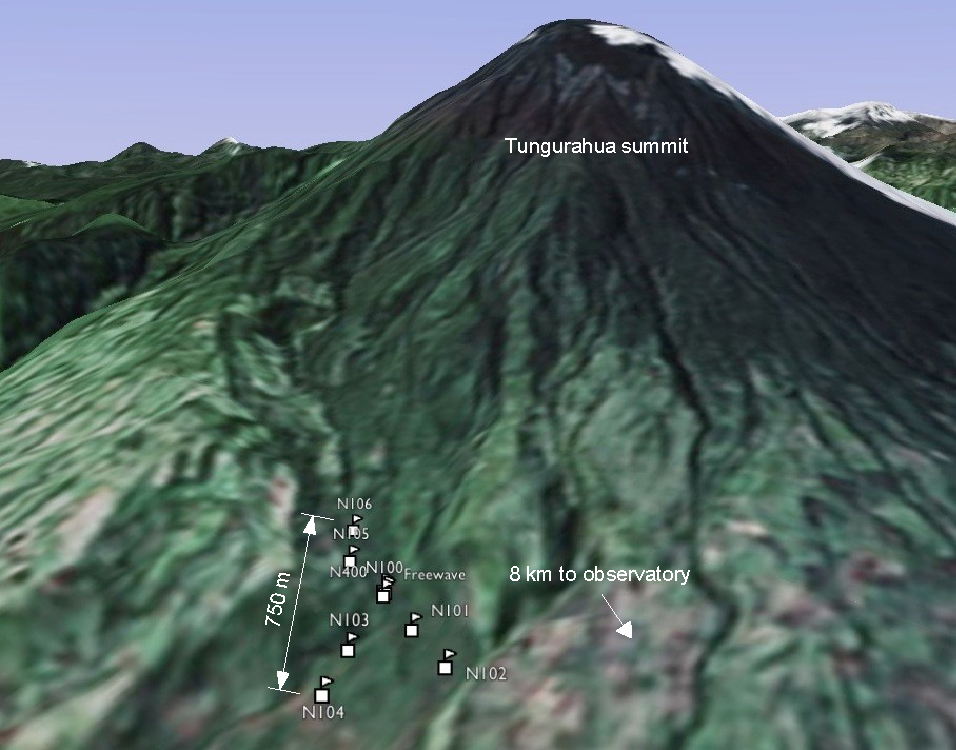
\includegraphics[width=0.7\hsize]{./4-lance/figs/map.pdf}
\end{center}

\caption{\textbf{Location of the Tungurahua sensor network deployment.}}

\label{lance-fig-map}
\end{figure}

As shown in Figure~\ref{lance-fig-map}, seven of the nodes were deployed in a
three-armed ``star'' topology radiating away from a central hub node, with
two nodes per arm. The eighth node was colocated with the hub and transmitted
an unreliable continuous stream of sensor data packets for establishing
ground truth. A separate gateway node relayed data (using a FreeWave radio
modem) to the base station laptop at the volcano observatory, 8~km from the
deployment site. Time synchronization was established using FTSP~\cite{ftsp}
with a single GPS receiver as the root of the synchronization tree. We
experimented with two summarization functions and several policy modules
during the field deployment.

\vfill\eject

\subsection{Overall Performance and Data Yield}

\begin{table}[t]
\begin{center}
\begin{tabular}{|l|l|l|} \hline
\textbf{Node}	& \textbf{ADUs downloaded} & \textbf{Mean throughput} \\ \hline
100 & 311 & 651.0 Bps \\
101 & 131 & 446.8 Bps \\
102 & 262 & 445.8 Bps \\
103 & 292 & 424.4 Bps \\
104 & 150 & 256.8 Bps \\
105 & 66 & 453.7 Bps \\
106 & 20 & 253.4 Bps \\ \hline
\textit{Total} & 1232 & 431.5 Bps \\ \hline
\end{tabular}
\end{center}

\caption{\textbf{Download performance during the deployment.}}

\label{lance-fig-throughput}
\end{table}

The sensor network was operational for a total of 71~hours, during which
Lance ran for a total of 56~hours. During this time, Lance successfully
downloaded 1232~ADUs, or 77~MB of raw data. An additional 308~downloads
failed due to timeout or stale summary information, for an overall success
rate of 80\%. 11012~unique ADU summaries were received from the network,
representing an aggregate of 688~MB of sampled data. Lance therefore
downloaded approximately 11\% of the data produced by the network.
Figure~\ref{lance-fig-throughput} summarizes the number of ADUs downloaded
and mean throughput for each node.

\begin{figure}[t]
\begin{center}
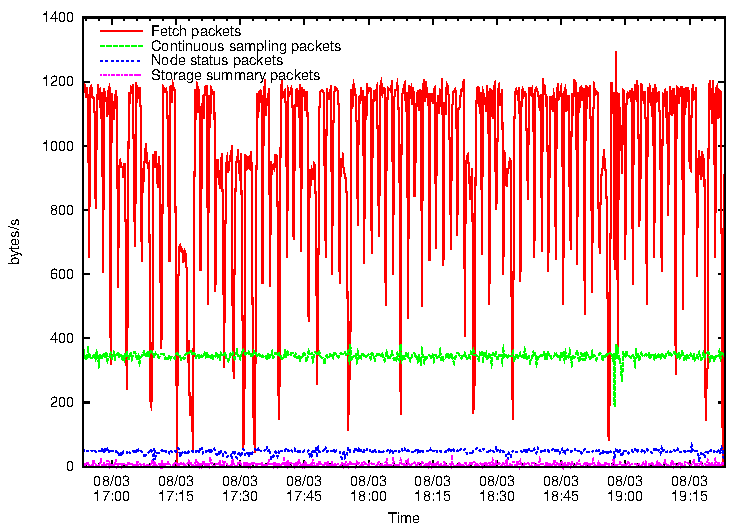
\includegraphics[width=0.9\hsize]{./4-lance/figs/packetgraph.pdf}
\end{center}

\caption{\textbf{Breakdown of radio traffic by packet type.} This figure
shows the total number of bytes received at the base station, averaged over
15~s intervals. Periodic node status messages and storage summaries comprise
a small fraction of the overall bandwidth.}

\label{lance-fig-packetgraph}
\end{figure}

Figure~\ref{lance-fig-packetgraph} shows a breakdown of the packets received
at the base station for a representative time period. Fetch download packets
consumed the majority of the bandwidth, followed by the continuous sampling
packets. The latter is a debugging feature allowing us to visualize the
seismic activity from a single node in real time, and is entirely optional.
Every node sent a periodic heartbeat to the base station every~10~s, and a
storage summary every 109~s. As the figure shows, this overhead is a small
percentage (less than 5\%) of the overall network traffic.

\subsection{RSAM-based Summarization}

\begin{figure}[t!]
\begin{center}
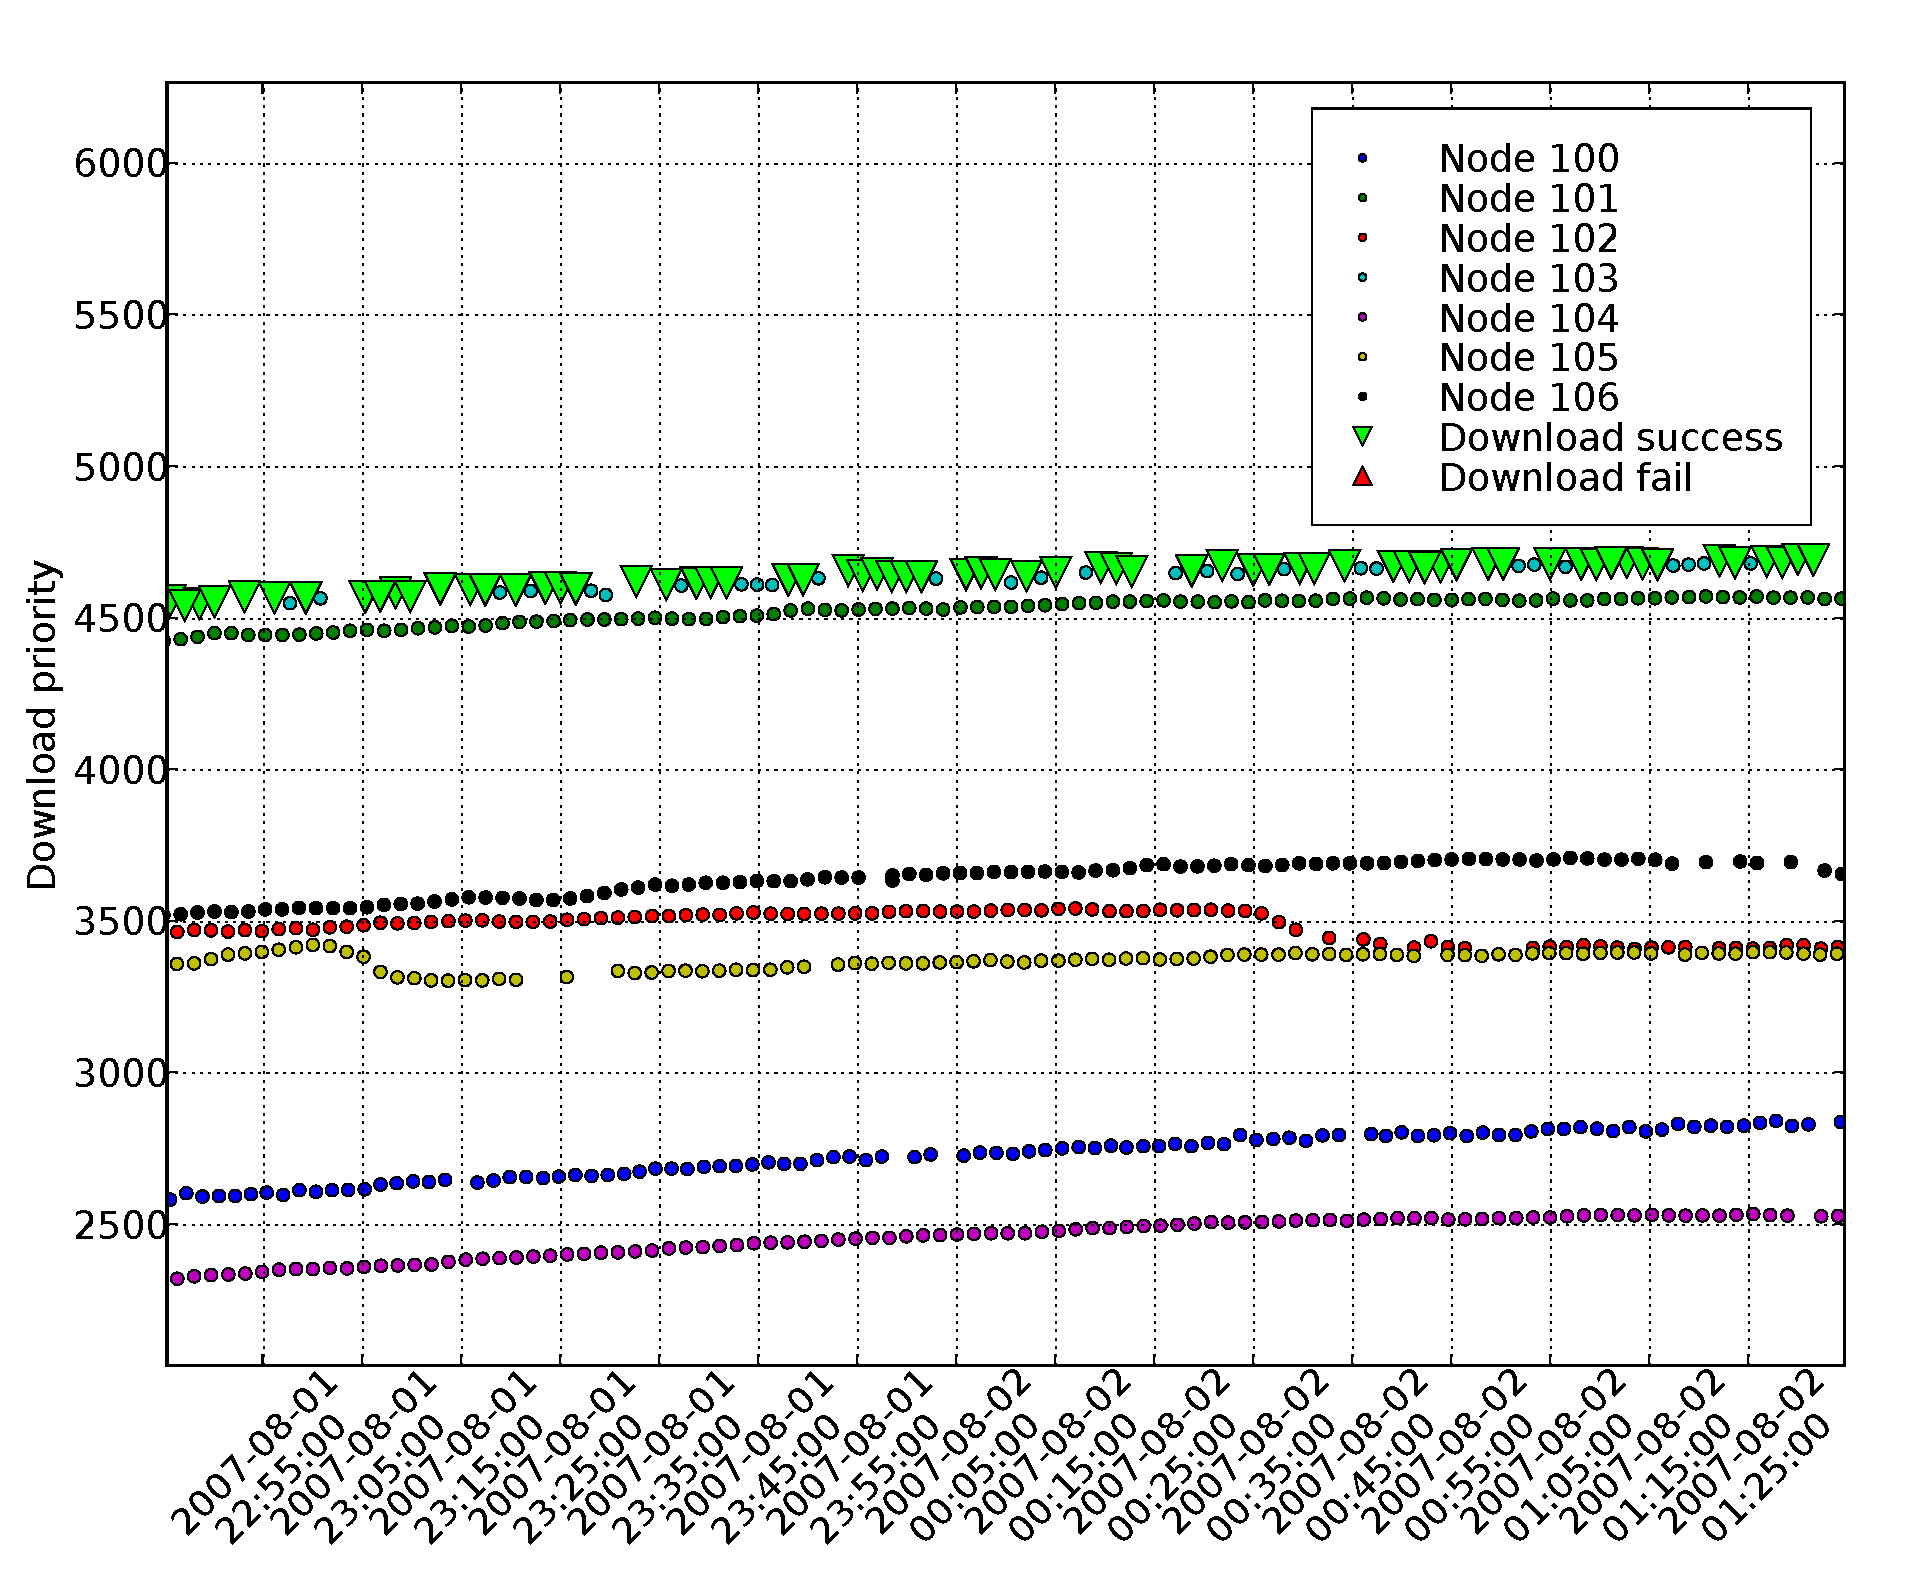
\includegraphics[width=0.8\hsize]{./4-lance/figs/dcbias.pdf}
\end{center}

\caption{\textbf{Effect of DC bias on RSAM summarization function.} Each
point represents the ADU value received at the base station, and the
triangles indicate those ADUs that were downloaded by Lance. Since nodes'
RSAM values are offset significantly from each other, Lance prefers
downloading from the node with the largest positive bias.}

\label{lance-fig-dcbias}
\end{figure}

The system as initially deployed computed the RSAM~\cite{rsam} as the value
for each ADU. This approach was intended to prioritize data based on the
overall level of seismic activity. We experienced two problems as soon as the
system was fielded. First, the RSAM calculation was sensitive to DC~bias in
the seismometer signal, causing Lance to generally prefer downloading ADUs
from one or two nodes (those with the largest positive bias).
Figure~\ref{lance-fig-dcbias} shows this effect, with Lance only downloading
ADUs from Node~103.

This problem was easily corrected, without any node software changes, by
introducing a policy module at the base station to process the raw RSAM
values received from each node and filter out the DC~bias. This was achieved
by computing the median RSAM value over each 30-minute window of raw RSAM
values on each node, and subtracting the median from the RSAM.

The second problem with the RSAM summarization function was caused by the
uncharacteristically low level of seismicity at the volcano throughout the
deployment. We observed only about 20~volcano-tectonic earthquakes and
\textit{no} clear explosions, whereas the previous week, Tungurahua exhibited
dozens of earthquakes each day. As a result, the RSAM summarization function
was generally unable to distinguish between actual seismic activity and
noise. We corrected this problem by switching to a different summarization
function (described below) that was designed to pick out small earthquakes.

To evaluate Lance's behavior with respect to an ``optimal'' system, we took
the 8483~RSAM summaries received during a 16-hour period when the debiasing
filter was enabled. Using this information, we compute the set of ADUs that
the optimal system would have downloaded, with complete knowledge of all ADUs
but limited to the same time duration the original network was operating. We
assume the download throughput for a given node is always the mean throughput
for that node observed during the deployment
(Figure~\ref{lance-fig-throughput}). This calculation ignores energy
constraints because the deployed system did not consider energy costs.

An optimal system would have downloaded 392~out of the~8483 ADUs, whereas the
actual system downloaded 418~ADUs during this time.\footnote{The optimal
system would download fewer ADUs than the real system due to the variation in
the throughput to each node: the optimal system would download more ADUs from
nodes with lower throughput, thereby limiting the total number of ADUs it
could download.} The total value of ADUs downloaded by the optimal system is
10678, whereas the value of the actual network was 10629, for an optimality
of 99.5\%. Lance did an exceptional job of extracting the highest-value data
from the network using our online heuristic algorithm.

\subsection{EWMA-based Summarization Function}
\label{lance-sec-ewma-deployment}

Given the low level of volcanic activity, after the first 25~hours of the
deployment we chose to reprogram the network to use the EWMA summarization
function (described in Section~\ref{lance-subsec-volcano}) which is designed
to pick out small earthquakes from background noise. Due to code size
limitations on the motes, it was necessary to manually reprogram each node
with the new summarization function, which took two teams about 4~hours.

This summarization function reports a high value for an ADU that appears to
contain an earthquake or other seismic event. However, there is no guarantee
that the event will be centered in the ADU: in the worst case, the earthquake
might occur at the very beginning or very end of the ADU, causing the initial
seismic P-wave arrival or waveform coda to be stored in adjacent ADUs with
low value. To avoid this problem, we made use of the \texttt{timespread}
policy module that detects ADUs with an elevated value (over a fixed
threshold) and assigns the immediately preceding and succeeding ADUs the same
value. By dilating the value over time, Lance should download all three of
the ADUs and maximize the probability that a given earthquake signal is
entirely downloaded.

As with the RSAM-based summarization function, we estimate the optimal set of
ADUs that an oracle would have downloaded. During a 25-hour period, the
network reported 11012~unique ADU summaries. An optimal system would have
downloaded 554 ADUs with total value 577377. The actual network downloaded
518~ADUs with a value of 539115, for an optimality of 93.3\%.

As a final evaluation metric, we wish to consider how well Lance, configured
in this manner, was able to download seismic signals representing
earthquakes. Given the low level of volcanic activity, it turns out that most
of the ADUs downloaded by Lance contain no discernible seismic signal. In
fact, upon manual inspection of the 518~ADUs downloaded during this period,
we identified only 20~ADUs showing a clear earthquake signal, corresponding
to only 9~separate seismic events. Note that we did \textit{not} configure
Lance to explicitly download correlated earthquakes as described in
Section~\ref{lance-sec-adaptation} so we would not expect a high degree of
coverage for the same event across multiple nodes.

\begin{figure}[t]
\begin{center}
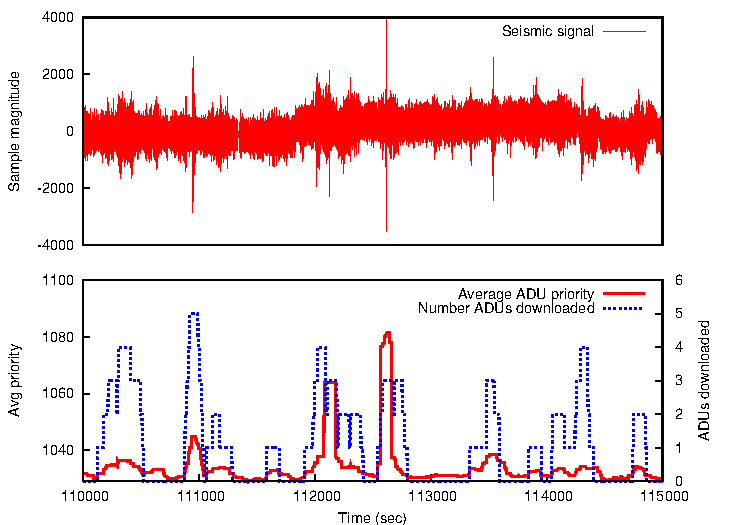
\includegraphics[width=1.0\hsize]{./4-lance/figs/everything.pdf}
\end{center}

\caption{\textbf{Lance download behavior overlaid with average ADU value.}
The top plot shows the continuous seismic signal collected by a single node.
The lower plot shows the average value of ADUs and the number of ADUs
downloaded for each window.}

\label{lance-fig-everything}
\end{figure}

Figure~\ref{lance-fig-everything} shows the behavior of Lance during a
representative 83-minute period. The figure breaks time into windows of
one-half an ADU duration (55~s in this case), and computed the mean ADU value
as well as the number of downloaded ADUs that overlap each time window. As
the data shows, elevated seismic activity is well-correlated with an increase
in the ADU value from across the network, as well as the number of downloaded
ADUs. Moreover, the few cases of clear seismic activity in the trace (at
times 111000, 112700, and so forth) tend to have more ADUs downloaded. Of the
9~separate seismic events, a total of 27~ADUs were downloaded, representing a
per-event ``coverage'' of 3~ADUs per event. This represents just under half
of the 7~nodes participating in the network.
